\documentclass[12pt, twocolumn]{article}
\usepackage[margin=3cm]{geometry}
\usepackage{listings}
\usepackage{graphicx}
\usepackage{float}
\usepackage{tikz}
\usepackage[justification=centering]{caption}
\usetikzlibrary{shapes.geometric,arrows}
\renewcommand{\lstlistingname}{\textbf{Program}}
\newcommand{\sanper}{\textsc{sanper-1 elu} }
%setting up flowcharts
\tikzstyle{startstop} = [rectangle, rounded corners, minimum width=3cm, minimum height = 1cm, text centered, draw=black, fill=red!30]

\tikzstyle{process} = [rectangle, minimum width=3cm, minimum height = 1cm, text centered, text width = 3cm, draw=black, fill=orange!30]

\tikzstyle{decision} = [diamond,  minimum width=1cm, minimum height = .5cm, text centered, text width = 2cm, draw=black, fill=green!30]

\tikzstyle{arrow} = [thick, ->,>=stealth]

\begin{document}

\begin{titlepage}
	\begin{center}
		
		
		% Upper part of the page. The '~' is needed because \\
		% only works if a paragraph has started.
		\vfill
		
		\textsc{\LARGE Experiment 4: Code Conversion and Bit Manipulation}\\[1.5cm]
		
		\Large Adam Sumner\\[0.5cm]
		
		\Large Illinois Institute of Technology\\[0.5cm]
		
		\Large ECE 441-01\\[0.5cm]	
		% Author and supervisor
		\noindent
		\vfill
		\large \textbf{Lab Date:} February 10th, 2015\hfill
		\large \textbf{Due Date:} March 3rd, 2015
		% Bottom of the page
		
		
	\end{center}
\end{titlepage}

\section{Introduction}
The purpose of this experiment is to:
\begin{itemize}
	\item Perform ASCII, BCD, and Hexadecimal code conversion
	\item Gain familiarity with the MC68k's bit manipulation instructions
	\item Learn how to download programs from a host computer and into the \sanper
\end{itemize}
The student will download a sample program into the \sanper and run it. A bit manipulation algorithm will then be developed and executed in the same manner of the sample program.
\section{Background}
The \sanper is capable of receiving MC68K programs from an external computer. Its downloading capability is achieved in hardware by connecting the serial port of the external source to one of the serial ports of the \textsc{sanper-1}. The download functionality is achieved via software through the TUTOR firmware. The external computer transmits a file through the serial port in S-Record format. 

Bit manipulation is the ability to modify each bit of a binary number according to some specified algorithm. The 68000 is equipped with four bit manipulation instructions:
\begin{itemize}
	\item \textit{BCHG} - Test a bit and change it
	\item \textit{BCLR} - Test a bit and clear it
	\item \textit{BSET} - Test a bit and set it
	\item \textit{BTST} - Test a bit 
\end{itemize}
It is also possible to manipulate bits with logical instructions such as:
\begin{itemize}
	\item \textit{AND} - Logical AND
	\item \textit{ANDI} - Logical AND Immediate
	\item \textit{OR} - Logical Inclusive OR
	\item \textit{ORI} - Logical Inclusive OR Immediate
	\item \textit{EOR} - Logical Exclusive OR
	\item \textit{EORI} - Logical Exclusive OR Immediate
	\item \textit{NOT} - Logical Compliment
\end{itemize}
Furthermore, bit manipulation can be performed with Shift and Rotate Instructions:
\begin{itemize}
	\item \textit{ASL} - Arithmetic Shift Left
	\item \textit{ASR} - Arithmetic Shift Right
	\item \textit{LSL} - Logical Shift Left
	\item \textit{LSR} - Logical Shift Right
	\item \textit{ROL} - Rotate Left
	\item \textit{ROR} - Rotate Right
	\item \textit{ROXL} - Rotate Left with Extend
	\item \textit{ROXR} - Rotate Right with Extend

\end{itemize}
\section{Equipment/Procedure}
\subsection{Equipment}
\begin{itemize}
	\item \textsc{SANPER-1 Educational Lab Unit}
	\item Computer with TUTOR software
\end{itemize}
\subsection{Procedure}
\begin{enumerate}
	\item Download the program located in Section \ref{sample} into the \sanper
	\item Execute the program and record results
	\item Download the program located in Section \ref{bitmanip} and execute it
	\item Verify results
\end{enumerate}

\section{Results}

This section shows the results of the terminal screen and the data display of the \sanper after running the bit manipulation program.

\begin{figure}[H]
\centering
\includegraphics[width=\linewidth]{tests}
\caption{Testing number input/output}
\label{fig:tests}
\end{figure}

\begin{figure}[H]
\centering
\includegraphics[width=\linewidth]{Exit}
\caption{Exit Functionality of Program}
\label{fig:Exit}
\end{figure}


\begin{figure}[H]
\centering
\includegraphics[width=0.8\linewidth]{FullSizeRender}
\caption{Input of 227}
\label{fig:FullSizeRender}
\end{figure}

\begin{figure}[H]
\centering
\includegraphics[width=0.8\linewidth]{FullSizeRender_1}
\caption{Input of 0}
\label{fig:FullSizeRender_1}
\end{figure}

\begin{figure}[H]
\centering
\includegraphics[width=0.8\linewidth]{FullSizeRender_2}
\caption{Input of 255}
\label{fig:FullSizeRender_2}
\end{figure}

\begin{figure}[H]
\centering
\includegraphics[width=0.8\linewidth]{FullSizeRender_3}
\caption{Input of 100}
\label{fig:FullSizeRender_3}
\end{figure}


\section{Discussion}

The bit manipulation program was developed by using the logic circuit shown below:
\begin{figure}[H]
\centering
\includegraphics[width=1\linewidth]{algorithm}
\caption{Bit Manipulation Logic}
\label{fig:algorithm}
\end{figure}

It was designed to continuously loop until the user entered the '.' character as input. The program takes the input number and stores it in memory. From here it performs an ASCII to decimal conversion by subtracting \$30 from the ASCII digit. This is because if you add \$30 to a decimal digit in hexadecimal, it produces the ASCII hex value. This can be shown in the characteristic table shown below:
\vspace{0.5cm}

\begin{center}
\begin{tabular}{|c|c|}
	\hline
	Decimal Number & ASCII Value(Hex)\\
	\hline
	1 & \$31 \\
	\hline
	2 & \$32 \\
	\hline
	3 & \$33 \\
	\hline
	4 & \$34 \\
	\hline
	5 & \$35 \\
	\hline
	6 & \$36 \\
	\hline
	7 & \$37 \\
	\hline
	8 & \$38 \\
	\hline
	9 & \$39 \\
	\hline
\end{tabular}
\end{center}

From this point, each digit of the input number is stored as a byte in memory. To convert from BCD to Binary, the number is multiplied by its corresponding 10's place and added to a data register that holds the final binary digit. After this, the binary number is manipulated due to the algorithm in Figure \ref{fig:algorithm}. To format for output to the terminal and the \sanper data display, the new number must be converted back to ASCII. This is done by converting it to BCD and then adding \$30 to each byte to get the ASCII hex value. The string is then outputted to the terminal, the number is formatted for the \sanper data display and placed in the correct output address. The program repeats until the user inputs the '.' character. This process is shown in Section \ref{flowchart}.

\section{Conclusion} 
Overall, this experiment was a success. ASCII, BCD, and Hexadecimal code conversion was accomplished, the bit manipulation instructions were explored, and programs were successfully downloaded to the \sanper.

\begin{thebibliography}{1}
	\bibitem{expman} Experiment 4 Lab Manual
	\bibitem{ecbm} Educational Computer Board Manual
	\bibitem{m68k}MC68K User Manual
	\bibitem{sanper}SANPER-1 ELU User Manual
	
	
\end{thebibliography}
  
\onecolumn
\section{Appendix}
\label{appendix}
\subsection{Flowchart of Bit Manipulation Program}\label{flowchart}
	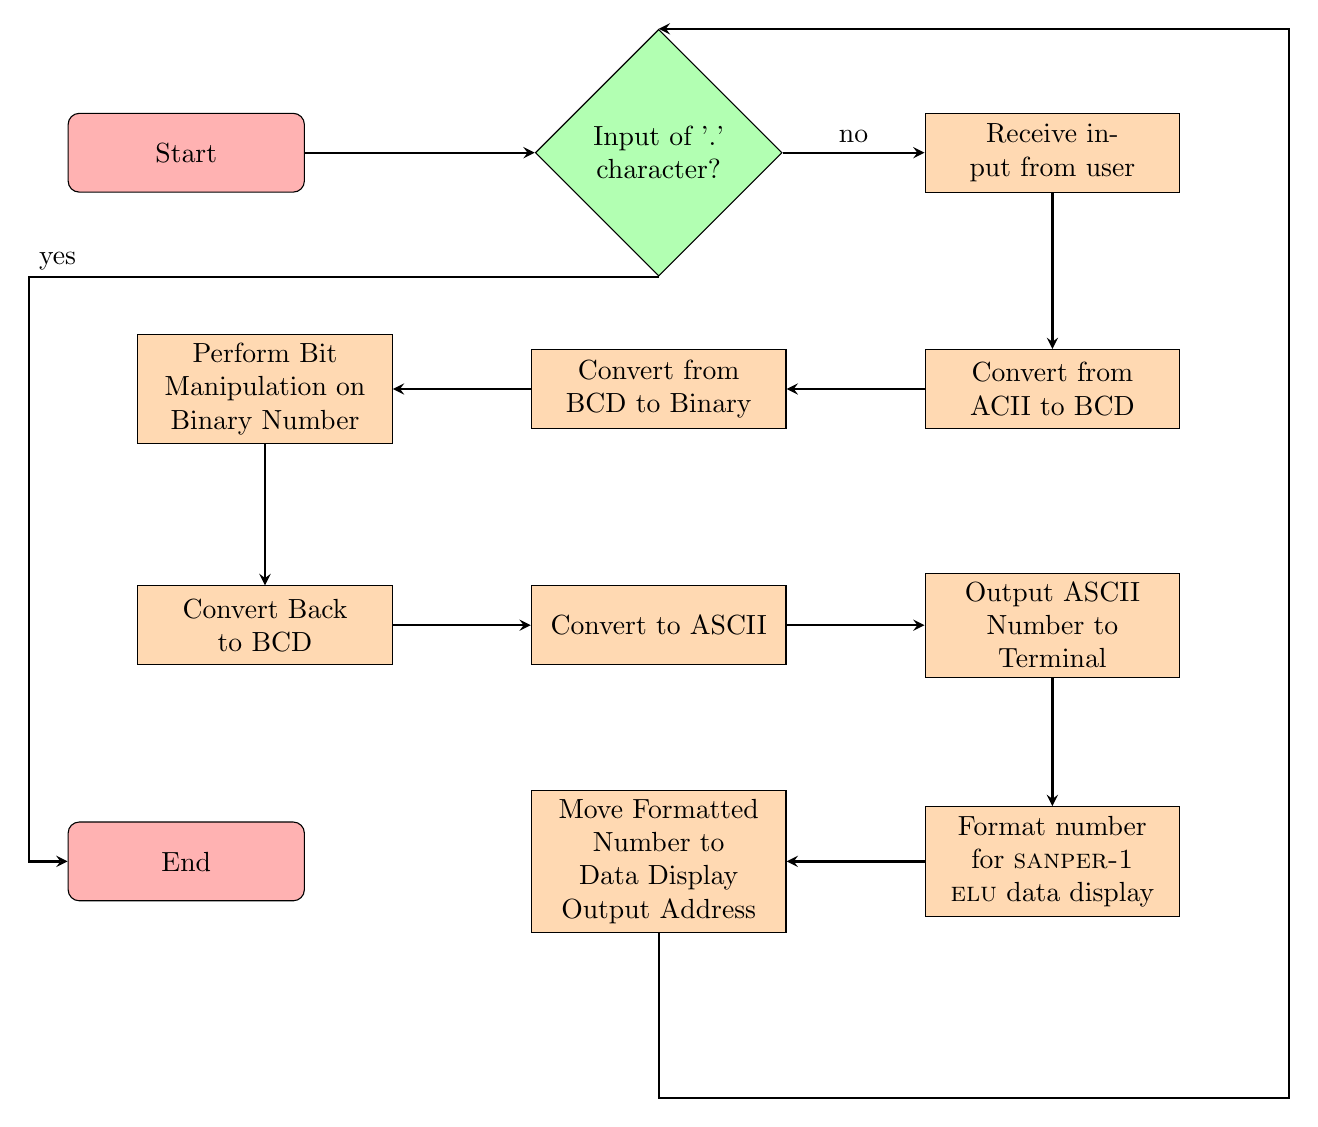
\begin{tikzpicture}[node distance = 2cm]
	\node (start) [startstop] {Start};
	\node (dec1)[decision, right of = start, xshift = 4cm]{Input of '.' character?};
	\node (pro1)[process, right of = dec1, xshift = 3cm]{Receive input from user};
	\node (pro2)[process, below of = pro1, yshift = -1cm]{Convert from ACII to BCD};
	\node (pro3)[process, left of = pro2, xshift = -3cm]{Convert from BCD to Binary};
	\node (pro4)[process, left of = pro3, xshift= -3cm]{Perform Bit Manipulation on Binary Number};
	\node (pro5)[process, below of = pro4, yshift = -1cm]{Convert Back to BCD};
	\node (pro6)[process, right of = pro5, xshift = 3cm]{Convert to ASCII};
	\node (pro7)[process, right of = pro6, xshift = 3cm]{Output ASCII Number to Terminal};
	\node (pro8)[process, below of = pro7, yshift = -1cm]{Format number for \sanper data display};
	\node (pro9)[process, left of = pro8, xshift = -3cm]{Move Formatted Number to Data Display Output Address};
	\node (end)[startstop, left of = pro9, xshift = -4cm]{End};		
	
	
	\draw [arrow] (start) -- (dec1);
	\draw [arrow] (dec1)--node[anchor = south] {no}(pro1);
	\draw [arrow] (pro1)--(pro2);
	\draw [arrow] (pro2)--(pro3);
	\draw [arrow] (pro3)--(pro4);
	\draw [arrow] (pro4)--(pro5);
	\draw [arrow] (pro5)--(pro6);
	\draw [arrow] (pro6)--(pro7);
	\draw [arrow] (pro7)--(pro8);
	\draw [arrow] (pro8)--(pro9);
	\draw [arrow] (dec1.south) -- ++(-8,0) node[anchor = west, yshift = 0.2cm]{yes} |-(end);
	\draw [arrow] (pro9.south)|-(14,-12)|-(dec1.north);		 
	\end{tikzpicture}
\subsection{Sample Program S-Records}
\begin{enumerate}
	\item 
	\begin{itemize}
		\item Type: S0
		\item Length: 21
		\item Address: 0000
		\item Data: 6384B50524F47202020323043524541544544204259204541535936384B
		\item Checksum: 6D
	\end{itemize}
	\item
	\begin{itemize}
		\item Type: S1
		\item Length: 0C
		\item Address: 0900
		\item Data: 495420574F524B5321
		\item Checksum: 76
	\end{itemize}
	\item 
	\begin{itemize}
		\item Type: S1
		\item Length: 23
		\item Address: 1000
		\item Data: 4FF82FFF4BF809004DF809091E3C00F34E4E1E3C00F14E4E1E3C00E34E4E60E4
		\item Checksum: C7
	\end{itemize}
	\item
	\begin{itemize}
	\item Type: S8
	\item Length: 04
	\item Address: 0000
	\item Data: 00
	\item Checksum: FB
	\end{itemize}
\end{enumerate}

\subsection{Code}\label{code}
\subsubsection{Sample Program}\label{sample}
\lstset{language=[Motorola68k]Assembler}
\lstinputlisting{4_1.X68}

\subsubsection{Bit Manipulation Program}\label{bitmanip}
\lstinputlisting{ASCII2DEC.X68}

\end{document}